\chapter{CryptID}

Az előző fejezetek előbb a kriptográfiai, majd a technológiai alapokat vezették be. Ebben a fejezetben a dolgozat eredményét jelentő programkönyvtár – a CryptID – kerül részletesen ismertetésre.

A fejezet felépítése a következő: Először magas szinten vázoljuk, hogy mi is pontosan a CryptID, miben jelent újdonságot, milyen megfontolások állnak mögötte. Ezt követi a könyvtár struktúrájának alapos bemutatása, rétegről rétegre haladva. Az utolsó előtti szekció egyfajta útmutatóként szolgál a CryptID felhasználásához, integrálásához. Végül a fejezetet a könyvtár teljesítményének elemzése zárja.


\section{Mi a CryptID?}

A CryptID egy nyílt forrású IBE megoldás, mely az RFC 5091-ben meghatározott Boneh-Franklin sémát veszi alapul. Újszerűsége két irányból is megközelíthető, egyrészt az implementációt, másrészt az IBE sémát tekintve. 

A megvalósításban rejlő újdonság, hogy a CryptID WebAssembly alapokon működik, aminek köszönhetően nemcsak a szerveroldalon, hanem a kliensoldalon, vagy akár a webtől teljesen elszakadva nyújt platformfüggetlen és hatékony titkosítási megoldást.

Az IBE sémához hozzátett újítás a publikus kulcsban keresendő. A CryptID strukturált publikus kulcsokra épül, melyekben az egyedi azonosítón felül tetszőleges metaadat elhelyezhető.

A következőkben az előbb felsorolt sajátosságokat fejtjük ki részletesen, mindenütt kitérve a háttérben álló motivációkra is.

\subsection{Platformfüggetlen működés}

A CryptID formájában egy olyan könyvtárat szerettünk volna létrehozni, mely hatékony kliensoldali titkosítást tesz lehetővé. Mindezt olyan formában szerettük volna megvalósítani, hogy ugyanaz a megoldás alkalmazható legyen asztali gépeken, tableteken és mobiltelefonokon egyaránt. Ezt az erőfeszítést az a motiváció hajtotta, hogy nem tudunk olyan nyílt forrású IBE könyvtárról, mely módosítás nélkül (\textit{out-of-the-box}) használható lenne ezen platformok mindegyikén.

Adott volt tehát a célkitűzés: egy böngészőben futtatható, hatékony programkönyvtár létrehozása. Korábban a JavaScript volt az egyetlen olyan technológia, mely ilyen mértékű platformfüggetlenséget kínált. Azonban az egyes böngészőkben található JavaScript motorok jelentősen eltérő optimalizációkat alkalmazhatnak, így ami az egyik böngészőben gyorsan fut, az elképzelhető, hogy egy másikban jóval gyengébb teljesítményt nyújt. Erre a problémára ugyan megoldást kínál az asm.js, mely egyszerűségénél fogva könnyebben és egyértelműbben optimalizálható, azonban ez korántsem tekinthető szilárd és jól támogatott szabványnak.

Rátaláltunk azonban az előző fejezetben ismertetett WebAssembly szabványra, mely pontosan azt nyújtotta, amire szükségünk volt: hordozható binárist és gyors végrehajtást. A WebAssemblynek köszönhetően kihasználhattuk azt is, hogy C-ben számos régóta fejlesztett és alaposan tesztelt matematikai, illetve kriptográfiai programkönyvtár áll rendelkezésre. Ilyen a GMP \cite{GMP} és az OpenSSL \cite{OpenSSL} is, melyek a CryptID alapját képzik.

\subsection{Strukturált publikus kulcs}

Az IBE lényege, hogy a publikus kulcs egy adott domainen belül valamilyen entitást egyértelműen azonosít. Legegyszerűbb példa erre egy email cím, vagy adott rendszeren belüli felhasználónév. Boneh és Franklin azonban a róluk elnevezett sémát leíró cikkükben \citeyear{Boneh::IdentityBasedEncryptionFromTheWeilPairing} említenek olyan alkalmazásokat is, melyek a publikus kulcsot további metaadatokkal egészítik ki. Ilyen metaadat lehet például az aktuális év, mely egyfajta érvényességet rendel a publikus kulcshoz és így áttételesen a hozzátartozó privát kulcshoz is. Az említett cikkben ez a metaadat egyszerűen az azonosítóhoz konkatenálva jelenik meg a publikus kulcsban: „\texttt{bob@company.com $\parallel$ current-year}”.

A metaadatok beágyazásának ötletét nagyszerűnek találtuk, azonban úgy éreztük, hogy a konkatenáció szükségtelen kötöttséget erőltet a publikus kulcsra: az egyes mezőknek mindig azonos sorrendben kell szerepelniük. Természetesen ezen közvetlenül nem változtathatunk, hiszen a titkosítás, majd a visszafejtés csak akkor működik az elvártnak megfelelően, ha a publikus kulcs mindig bitpontosan azonos.

E megszorítást csak az absztrakció szintjének megemelésével kerülhettük meg. A \mbox{CryptID} ennek folytán JavaScript objektumokat használ publikus kulcsként. Az objektumok publikus kulcsra történő leképezése a könyvtár implementációs részletei közé tartozik, ezzel a CryptID-et integráló fejlesztőnek nem kell foglalkoznia. Ily módon a CryptID megszünteti a sorrendi kötöttség okozta terhet, mi több, a fejlesztőknek azzal sem kell törődniük, hogy a publikus kulcsot reprezentáló objektumból hogyan lesz bitsorozat – a konverzió a kulisszák mögött történik.

\subsection{Nyílt forrású, RFC-alapú implementáció}

Egy adott kriptorendszerhez megbízható implementációt készíteni rendkívül nehéz feladat. Hiába áll ugyanis rendelkezésünkre egy matematikailag bizonyítottan biztonságos kriptorendszer, annak megvalósítása során könnyen véthetünk olyan hibákat, melyek sebezhetőségeket nyitnak. Ezek a sebezhetőségek fakadhatnak például programozási hanyagságból (például a bemenet nem megfelelő ellenőrzése), vagy matematikai figyelmetlenségből, tudatlanságból (támadható elliptikus görbe használata).

Számos gyakori hiba megelőzhető azonban, ha valamilyen nyílt szabvány vagy ajánlás alapján készítjük el az implementációnkat. A CryptID esetében is így tettünk: az RFC 5091-et használtuk fel, mely a Boneh-Franklin és a Boneh-Boyen IBE rendszerek lehetséges implementációját írja le egy bizonyos szuperszinguláris elliptikus görbe felett \cite{RFC5091}. Ezek közül a CryptID a Boneh-Franklin rendszerre épül.

Az említett RFC részletes pszeudokódot biztosít az IBE-t felépítő főbb algoritmusokhoz (\textit{Setup, Extract, Encrypt, Decrypt}, és alacsonyabb szintű társaik), ajánlásokat ad öt biztonsági szintre vonatkozóan (vö. \dotref{table::RFC::SecurityParam} táblázat), lehetővé téve ezzel a rendszer parametrizálását, valamint tesztadatokat tartalmaz, melyek elősegítik az implementációk tesztelését. Ezek a tesztadatok hatalmas segítséget jelentettek a fejlesztés során, hiszen a teljes rendszer lekódolása előtt meg tudtunk bizonyosodni az azt felépítő kisebb rutinok helyes működéséről is.

A CryptID nemcsak az ajánlásnak megfelelő, hanem egyúttal nyílt forrású is. Természetesen a nyílt forrású szoftverek nem lesznek automatikusan biztonságosabbak, mint zárt forrású társaik, azonban a transzparenciának köszönhetően a kód könnyebben és többek által átvizsgálható és ellenőrizhető, így összességében a nyílt forrás hozzájárulhat a megbízhatóbb implementáció létrejöttéhez \cite{Wheeler::SecureProgrammingForLinuxAndUnixHOWTO}.

\pagebreak


\section{A CryptID felépítése}

Magas szintről szemlélve, a CryptID három komponensből áll:

\begin{outdentlist}
    \item[]\textbf{CryptID.ref.}
    Java nyelven írt referencia-implementáció. Az egyetemi tanulmányaink során leggyakrabban a Java nyelvvel volt alkalmunk dolgozni, ennek folytán Javaban rendelkezünk a legmagabiztosabb tudással. Ezt kihasználva, először elkészítettük az IBE Java nyelvű megvalósítását, melyet aztán felhasználhattunk a WebAssembly implementáció helyességének ellenőrzéséhez.

    \item[]\textbf{CryptID.wasm.}
    Az IBE-t alkotó rutinokat tartalmazó WebAssembly modul. A forrásnyelv C, ezt fordítjuk át Emscripten segítségével WebAssemblyre (ld. \dotref{Subsection::WebAssembly::Forditas}).

    \item[]\textbf{CryptID.js.}
    A WebAssembly modult becsomagoló JavaScript könyvtár, mely egy könnyen használható interfészen keresztül teszi elérhetővé az IBE rutinokat.
\end{outdentlist}

E három komponens valójában két különálló, bár szemantikát tekintve azonos IBE-megoldást alkot. Az egyiket a CryptID.ref önmagában, míg a másikat a CryptID.wasm és arra építve a CryptID.js. A továbbiakban a CryptID.ref ismertetését elhagyjuk, és a CryptID néven a CryptID.wasm és a CryptID.js komponensek együtteséből formált könyvtárra fogunk hivatkozni. E könyvtár struktúráját az \dotref{Figure::CryptID::Stack} ábra szemlélteti.

\begin{figure}[h]
    \centering
    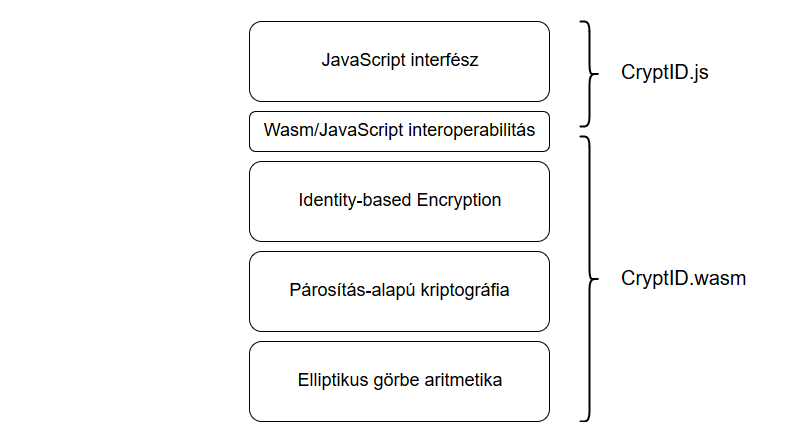
\includegraphics[height=225px]{05-cryptid/stack-smaller-gaps-box-centered.png}
    \caption{A CryptID felépítése.}
    \label{Figure::CryptID::Stack}
\end{figure}

A következőkben lentről felfelé haladva részletesen bemutatjuk az egyes rétegeket.

\subsection{Elliptikus görbe aritmetika}

Az IBE egy elliptikus görbe kriptográfián alapuló titkosítási rendszer, ezért az elliptikus görbe aritmetika képzi a CryptID magját is. A \ref{Chapter::ECC}. fejezetben összefoglaltuk az elliptikus görbék legfontosabb matematikai tulajdonságait, dolgozatunk ezen részében pedig az implementációhoz szükséges ismereteket tárgyaljuk.

Az elliptikus görbék matematikai háttere hosszú múltra tekint vissza, és számos elliptikus görbe aritmetikát megvalósító könyvtár áll rendelkezésre. Természetesen merül fel a kérdés, hogy ezek ellenére miért készítettünk saját implementációt?

Úgy találtuk, hogy az általunk vizsgált könyvtárak mindegyike rendelkezett olyan negatív tulajdonsággal (jelentős méret, átláthatatlan implementáció, hiányos dokumentáció), ami miatt úgy döntöttünk, hogy egy saját, pehelysúlyú réteget hozunk létre, ami megfelel minden elvárásunknak.

\subsubsection{Elliptikus görbe aritmetika tulajdonságai}

Az elliptikus görbe aritmetikát megvalósító rétegnek a legfontosabb tulajdonsága, hogy az RFC 5091-ben ajánlott \textit{Type-1} elliptikus görbékre van optimalizálva. A \textit{Type-1} osztály olyan görbéket takar, melyek alakja $E(\mathbb{F}_p) : y^2 = x^3 + 1$, ahol  $p \equiv 11 (\bmod \; 12)$ tetszőleges prím. Ezek a görbék a szuperszinguláris görbék egy részcsoportját képezik.

Az $\mathbb{F}_p$-beli elemek ábrázolására a GMP aritmetikai könyvtár véges test támogatását használtuk fel, ami egy rendkívül kiforrott és jól tesztelt megoldást nyújt.

A réteg képes $\mathbb{F}_{p^2}$-beli elemek ábrázolására is, amelyek lényegében $\mathbb{F}_p$-beli elemek rendezett párjai. Egy ilyen rendezett párt jelölünk $(a_0, a_1)$-el, amit értelmezhetünk az $a_0 + a_1 \cdot i$ komplex számnak, ahol $i^2 = -1$. 

Ezzel az értelmezéssel egyszerűen a komplex aritmetikát alapul véve végezhetünk műveleteket $\mathbb{F}_{p^2}$ felett, annyi különbséggel, hogy minden esetben moduloját kell venni az eredményeknek, hogy a műveletek zártak maradjanak. Az ilyen műveletek kivitelezését a GMP alapú $\mathbb{F}_p$ test feletti aritmetikára építve végeztük el. 

Implementálásra került $\mathbb{F}_{p^2}$ feletti elemek egymással és skalárral vett összeadása, additív inverz képzése, elemek egymással és skalárral való szorzása, hatványozása egész számmal és multiplikatív inverz képzése.

Az említett $\mathbb{F}_{p^2}$ aritmetika implementálására azért volt szükség, mert a kriptográfiában az egyszerű Tate párosítás gyakran nem alkalmazható. Ugyanakkor, ha módosítjuk annyiban, hogy az egyik bemenete egy torzítási leképezése az elliptikus görbe egy pontjának, akkor biztosan két egymástól lineárisan független ponttal dolgozhatunk, kizárva az elfajultságot.

\subsubsection{Elliptikus görbe pontjainak ábrázolása}

A réteg két lehetőséget nyújt a görbe pontjainak ábrázolására. Egyik az affin térben való ábrázolás, a másik lehetőség pedig a projektív tér használata. Egy alap IBE implementációhoz elegendő lenne az affin pontábrázolás is, azonban a projektív koordináták használata egyszerű optimalizációs lehetőségeket nyújt.

Fontos megjegyezni, hogy több módja is van a projektív pontábrázolásnak, melyek közül mi az RFC 5091 ajánlását követve a Jacobi projektív módszert implementáltuk. Amíg az affin ábrázolás esetében a pontunkat egy $(x, y)$ számpáros alkotja, a Jacobi projektív módszer egy $(x, y, z)$ számhármast használ.

Miben is rejlik az utóbbi módszer hatékonysága? Nos, ha $M, S$ és $I$ rendre a szorzás, négyzetre emelés és invertálás műveleteit jelölik, akkor az \dotref{table::OperationCost} táblázatban látható, hogy az egyes módszerek és görbe műveletek esetén melyik test-műveletet hányszor kell végrehajtani.

A lényegi különbséget az invertálás elhagyása jelenti a görbe műveletek esetén, mert a szorzás és invertálás számításigényének aránya általánosan $80 : 1$ \cite{Nyakacska::ECC-PBC}, míg a szorzás és négyzetre emelés esetén $10 : 8$ \cite{BernsteinLange::ECC}.

\begin{table}[H]
    \centering
    \begin{tabular}{|l|l|l|}
    \hline
    \textbf{Pontábrázolás típusa} & \textbf{Összeadás} & \textbf{Duplázás} \\ \hline
    affin                         & $I + 2M + 2S$      & $I + 2M + 1S$     \\ \hline
    Jacobi projektív              & $12M + 4S$         & $4M + 6S$         \\ \hline
    \end{tabular}
    \caption{Elliptikus görbén végzett műveletek költsége \protect\cite{Martin::IntroductionToIdentityBasedEncryption}.}
    \label{table::OperationCost}
\end{table}

A tárgyalt ábrázolási módok mindegyikével a következő elliptikus görbe műveletek végezhetők:

\begin{outdentlist}
    \item[]\textbf{Pont duplázás.}
    Egyszerű pont duplázást megvalósító algoritmus, melyet a Martin könyvében leírtak alapján implementáltunk.
    
    \item[]\textbf{Pont összeadás.}
    Az implementált algoritmus forrása megegyezik a duplázás esetében használttal.

    \item[]\textbf{Pont szorzása skalárral.} 
    A \textit{Double-and-Add} algoritmust megvalósító skaláris szorzás került implementálásra a rétegben, ami megfelelőnek mondható, de még optimalizálható sebességet nyújt.
    
    \item[]\textbf{Pontábrázolások közötti konverzió.}
    A réteg részét képezi a két említett pontábrázolás közötti konverzió, ami affinból Jacobi projektívbe való átalakítás esetén $(x, y) \rightarrow (x, y, 1)$, fordított irányban pedig $(x, y, z) \rightarrow (x/z^2, y/z^3)$ módosítást végez.
\end{outdentlist}

\subsection{Párosítás-alapú kriptográfia}

A BF-IBE-nek és így a CryptID-nek is kihagyhatatlan része a párosítás műveletének megvalósítása. Az RFC 5091 ajánlását követve a réteg a Tate párosítást tartalmazza.

Az implementált Tate párosítás két $E(\mathbb{F}_p)$-beli pontot képez le egy $\mathbb{F}_{p^2}$-beli elemre. Az implementációt az RFC 5091 \citeyear{RFC5091}, Martin könyve \citeyear{Martin::IntroductionToIdentityBasedEncryption} és Lynn doktori disszertációja \citeyear{Lynn::PBC} alapján készítettük el.

\subsection{Identity-based Encryption}

A CryptID fő funkcionalitását megvalósító réteg. Tartalmazza a BF-IBE négy fő függvényét (\textit{Setup}, \textit{Extract}, \textit{Encrypt}, \textit{Decrypt}), amelyeket az Identity-based Encryption című fejezetben ismertettünk.

Az implementáció során az RFC 5091 ajánlásait követtük, amelyek nem csupán az említett függvénynégyesre vonatkoznak, hanem az azok működtetéséhez szükséges algoritmusokra is. 

Ilyenek az Identity-based Encryption című fejezet pszeudokódjaiban megjelent hash függvények:

\begin{outdentlist}
    \item[]\textbf{H1 - \textit{hashToPoint}} $\{0, 1\}^* \rightarrow G_1$
    
    \item[]\textbf{H2 - \textit{canonical}} $G_\mathbb{T} \rightarrow \{0, 1\}^n$
    
    \item[]\textbf{H3 - \textit{hashToRange}} $\{0, 1\}^n \times \{0, 1\}^n \rightarrow \mathbb{Z}_q$
    
    \item[]\textbf{H4 - \textit{hashBytes}} $\{0, 1\}^n \rightarrow \{0, 1\}^n$
\end{outdentlist}

A felsorolt hash függvények alapját a \textit{canonical} kivételével a Secure Hash Algorithms (SHA) hash függvény alkotja, amelyet számunkra az OpenSSL könyvtár biztosított. Az előbbi könyvtárat nem csupán az SHA implementációja miatt használjuk, hanem a kriptográfiailag biztonságos és jól tesztelt random szám generátora is nagy segítséget nyújtott számunkra.

\subsection{Wasm/JavaScript interoperabilitás}

A megelőző három réteg együttesen egy C nyelvű IBE implementációt alkot, mely akár WebAssemblyre történő fordítás nélkül is felhasználható, például natív alkalmazások készítéséhez. Természetesen a CryptID-ben nem mint natív könyvtár, hanem mint WebAssembly modul kerülnek elhelyezésre ezek a rétegek, egy JavaScript interfész mögé rejtve.

Felmerülhet a kérdés, hogy miért szükséges egy ilyen absztrakció, ha egyszer a WebAssemblyt beágyazó környezetek közvetlenül is lehetővé teszik a modulban definiált függvények meghívását? A válasz erre kettős: Egyfelől nincsen rá szükség, a CryptID.wasm önmagában is felhasználható. Másfelől viszont, a CryptID-et elsősorban olyan beágyazó környezetekben történő felhasználásra szánjuk, melyek JavaScripten keresztül teszik lehetővé a WebAssembly modulok meghívását. Ilyen környezet például a böngésző vagy a Node.js. Ezekben a környezetekben nagy segítséget jelent, hogy a CryptID ugyanúgy hívható, mint bármely más, JavaScriptben írt könyvtár, a WebAssembly pedig csupán implementációs részlet marad. 

E megközelítés támogatásához, még a JavaScript interfész alatt megtalálható egy úgynevezett interoperabilitási (röviden: interop) réteg, melynek egyik fele C-ben, másik fele pedig JavaScriptben készült. Az említett réteg a következő feladatokat látja el:

\begin{outdentlist}
    \item[]\textbf{C függvények becsomagolása.}
    Ahhoz, hogy a C-ben írt függvények JavaScriptből hívhatók legyenek, be kell csomagolni őket az Emscripten által biztosított \texttt{Module} objektum \texttt{cwrap} metódusa segítségével. Az interop réteg gondoskodik a WebAssembly-oldalon exportált összes függvény helyes becsomagolásáról.

    \item[]\textbf{Adattípusok közötti konverzió.}
    A C-ben készült IBE függvények két olyan adattípust is felhasználnak, melyek konverziót igényelnek:

    \begin{itemize}
        \item
        Míg a JavaScript-oldal a nagy egészeket karakterláncok formájában kezeli (adott számrendszerben reprezentálva az értéket), addig C-ben a GMP könyvtár \texttt{mpz\_t} típusa használatos. E két típus között kétirányú konverzióra van szükség (hiszen a nagy egészek kimenetet és bemenetet is jelenthetnek), melyet a GMP \texttt{mpz\_get\_str}\footnote{\url{https://gmplib.org/manual/Converting-Integers.html#Converting-Integers}} és \texttt{mpz\_init\_set\_str}\footnote{\url{https://gmplib.org/manual/Simultaneous-Integer-Init-_0026-Assign.html}} függvényeinek felhasználásával valósítottunk meg.

        \item
        A titkosítást implementáló C függvény a \texttt{CipherTextTuple} típus egy példányát állítja elő, mely nyers bájtsorozatokat is tartalmaz. Habár JavaScriptben az \texttt{ArrayBuffer}\footnote{\url{https://developer.mozilla.org/en-US/docs/Web/JavaScript/Reference/Global_Objects/ArrayBuffer}} lehetővé teszi a bináris adatok hatékony kezelését, azonban a továbbítás vagy mentés legtöbbször nem nyers formában történik. Ennek elősegítésére az interop réteg Base64 kódolásúra\footnote{\url{https://tools.ietf.org/html/rfc4648#section-4}} alakítja a \texttt{CipherTextTuple} bináris tartalmát.
    \end{itemize}

    \item[]\textbf{Kétirányú adatáramlás biztosítása.}
    A WebAssembly modulok egy vagy több elkülönített, lineáris memóriát használhatnak \cite{WebAssemblySpecification}. A böngészőben történő beágyazás esetében ezek a memóriaterületek a JavaScript kód által használt memóriától izoláltan kerülnek lefoglalásra. Mivel közvetlenül nem lehetséges az összetett típusok (például a különböző \texttt{struct} típusok) paraméterként vagy visszatérési értékként való használata, ezért ezen típusok példányait csak a WebAssembly és a JavaScript által birtokolt memóriaterületek közötti másolással lehet kicserélni. Ennek megfelelő lebonyolítása magában foglalja a lineáris memória JavaScript oldalról történő írását és olvasását, valamint a C oldalon történő helyes memóriafoglalást és -felszabadítást.
\end{outdentlist}

\subsection{JavaScript interfész}

A JavaScript interfész jelenti a CryptID külvilág számára nyilvános függvényeit és adattípusait. Míg a megelőző rétegek implementációs részletnek tekinthetők, addig erre az interfészre a kliensek közvetlenül is támaszkodhatnak. 

\subsubsection{Felelősségi körök}

Azon felül, hogy az interfész kapcsolatot jelent a könyvtár alsóbb rétegei és az integráló kliens között, további felelősségi köröket is ellát:

\begin{outdentlist}
    \item[]\textbf{A bemenet ellenőrzése.}
    Mivel ez a réteg választja el a könyvtár megvalósítását a külvilágtól, ez az egyetlen olyan pont, ahol hibás adatok léphetnek be a rendszerbe. Ilyen hibás bemenetre számtalan példa adható, elég ha a \texttt{null} értékekre, a nem megfelelő alakú objektumokra vagy a hibásan kódolt adatokra gondolunk. Az ilyen rendellenes inputok kiszűrése ebben a rétegben történik, mielőtt még bármilyen számítás alapját képezhetnék.

    \item[]\textbf{Kulcskonverzió.}
    A CryptID jelentette újdonságok közül az egyik a strukturált, metaadatokat tartalmazó publikus kulcs, melyet a könyvtár egy JavaScript objektum formájában vár. Fontos követelmény azonban, hogy a tartalmilag azonos JavaScript objektumokból mindig azonos bitsorozatot kell előállítani.
    
    Naiv megoldása lehetne ennek a problémának a következő: először a \texttt{JSON.stringify} függvény segítségével karakterláncot képzünk az objektumból, majd ezt egyszerű bitsorozatként interpretáljuk (azaz \texttt{char[]} típusként C-ben). E megközelítés azonban tartalmilag azonos objektumok esetén eltérő karakterláncokat eredményezhet, abból kifolyólag, hogy a \texttt{JSON.stringify} az objektumok kulcsait azok hozzáadásának sorrendjében konvertálja \cite{ECMAScript2015Specification}.
    
    Ezt megkerülendő, a \texttt{JSON.stringify} meghívása előtt a CryptID a publikus kulcsként szolgáló objektumból létrehoz egy vele tartalmilag azonos objektumot, melyhez azonban a kulcsok betűrendben kerülnek hozzáadásra. E konverziónak köszönhetően a JavaScript interfész alatti rétegek már egy bitsorozatot kapnak publikus kulcsként, a strukturáltsággal tehát egyáltalán nem kell foglalkozniuk.
\end{outdentlist}

\subsubsection{Exportált típusok}

A JavaScript interfész által exportált összes típus WebIDL\footnote{\url{https://www.w3.org/TR/WebIDL-1/}} definíciója megtalálható a CryptID – WebIDL definíciók függelékben,
% ref majd hozzá
a tényleges funkcionalitást biztosító két interfész azonban a könnyebb áttekinthetőség kedvéért az \dotref{Listing::CryptID::WebIDLInterfaces} kódrészletben is megtalálható.

\lstinputlisting[language=WebIDL, caption={A funkcionalitást biztosító interfészek.}, captionpos=b, label=Listing::CryptID::WebIDLInterfaces, firstline=1, lastline=21]{./code/cryptid.webidl}

Az integráló kód számára a könyvtár a \texttt{CryptIDFactory} interfész példányaként jelenik meg. Ezen interfész egyetlen függvénye az objektumgyárként (\textit{factory}) funkcionáló \texttt{getInstance}, mely a \texttt{CryptID} példányok aszinkron létrehozására képes. A \textit{factory} metódus által biztosított indirekció lehetővé teszi, hogy a visszaadott interfész mögé más és más implementáció kerüljön; például WebAssemblyt nem támogató böngésző esetén egy asm.js megvalósítás. Az aszinkronitás pedig annak enged utat, hogy a hívó kód futása a példány előállítása közben is folytatódhasson. E módon lehetséges például a WebAssembly kód lusta (\textit{lazy}) betöltése: a Wasm bináris nem kerül letöltésre a weboldal többi részével együtt, hanem csak a \texttt{getInstance} függvény meghívásakor indul el a háttérben a letöltés, feldolgozás és validálás.

Az IBE-hez kapcsolódó rutinokat a \texttt{CryptID} interfészen találjuk. E függvények visszatérési értéke minden esetben tartalmaz egy \texttt{success} nevű mezőt, mely a kívánt művelet sikerességét jelzi. Ha például a \texttt{decrypt} metódust nem a megfelelő privát kulccsal hívjuk, akkor a visszaadott objektum \texttt{success} mezője \texttt{false} értéket fog felvenni. Azért választottuk ezt a megoldást a kivételekkel szemben (és valójában mellett), mert a kivételeket valóban a kivételes esetek számára tartjuk fent \cite{Bloch::EffectiveJava}, mint például a hibás bemeneti formátumok, a megsértett invariánsok vagy a váratlan számítási hibák. Úgy gondoljuk, hogy e módon egy könnyebben integrálható, kényelmesebb felületet tudunk biztosítani a kliensek számára.

Érdemes még megemlíteni a \texttt{dispose} függvényt, mely a \texttt{CryptID} interfész által lefoglalt erőforrások elengedésére, felszabadítására szolgál. Ilyen erőforrás lehet például a WebAssembly implementáció esetén a modul által használt memóriaterület. Ha már nincs szükségünk IBE rutinokra, akkor érdemes a \texttt{dispose} segítségével a lehető leghamarabb felszabadítani a nem használt erőforrásokat. A \texttt{dispose} hívását követően bármelyik, az adott példány által biztosított függvény meghívása (beleértve magát a \texttt{dispose}-t is) hibának számít, és kivételt eredményez. 

\section{Alkalmazásfejlesztés CryptID-del}
\label{Section::CryptID::ApplicationDevelopment}

A következőkben a könyvtár alapszintű felhasználását mutatjuk be egy JavaScript program formájában. Ennek célja, hogy illusztrálja a CryptID integrálásának egyszerű voltát. A könnyebb olvashatóság érdekében a programot kisebb kódrészletekre bontva ismertetjük, a CryptID – Példaprogram függelékben
% megfelelő hivatkozás
azonban egyben is megtalálható a teljes forráskód.

Előbb a biztosított funkcionalitás rövid leírását adjuk, amit aztán a forráskód és az ahhoz fűzött magyarázatok követnek. 

\subsection{Funkcionalitás}

A példaprogram által megvalósított funkcionalitás a következő: Először új nyilvános paramétereket és mesterkulcsot generál. Ezt követően egy előre rögzített üzenetet titkosít egy email címet tartalmazó nyilvános kulccsal. A titkosítás után előállítja a nyilvános kulcshoz tartozó privát kulcsot, végül pedig ennek használatával visszaállítja az eredeti üzenetet a titkos szövegből.

\subsection{Implementáció}

\textit{Szeretnénk felhívni a figyelmet arra, hogy az olvashatóság megőrzése érdekében a következő kódrészletek nem tartalmaznak hibakezelést. Ezen felül kiemelnénk, hogy a sorok számozása folytonos, azaz a mindenkori sorszám a teljes forrásban elfoglalt pozíciót tükrözi.}

\lstinputlisting[language=JavaScript, firstline=1, lastline=2, escapechar=^]{./code/application-development-with-cryptid.js}

Az első teendőt a felhasznált könyvtárak importálása jelenti. A \texttt{perf\_hooks} a futási idő mérésére szolgáló rutinokat biztosít, míg a a \texttt{cryptid} a korábban említett \texttt{CryptIDFactory} interfész egy példányát exportálja.

\lstinputlisting[language=JavaScript, firstline=4, lastline=7, escapechar=^, firstnumber=4, showstringspaces=false]{./code/application-development-with-cryptid.js}

Mind az üzenet, mind a publikus kulcs rögzített értékkel bír. A publikus kulcs egy JavaScript objektum, mely metaadatokat ezúttal nem, csupán egy azonosításra használható email címet tartalmaz. Ennek valódi szerepe ugyanakkor jelenleg nincsen, hiszen az azonosító ellenőrzése nem része a példaprogramnak.

\lstinputlisting[language=JavaScript, firstline=9, lastline=10, escapechar=^, firstnumber=9, showstringspaces=false]{./code/application-development-with-cryptid.js}

Az IBE függvények a \texttt{CryptID} interfészen találhatók, melynek példányait a \texttt{CryptIDFactory} interfész által definiált \texttt{getInstance} metódus képes előállítani. Ennek végrehajtása aszinkron, ezért a JavaScript \texttt{async-await} szintaxisát használjuk a visszatérési érték kinyeréséhez.

\lstinputlisting[language=JavaScript, firstline=12, lastline=15, escapechar=^, firstnumber=12, showstringspaces=false]{./code/application-development-with-cryptid.js}

Amennyiben még nem rendelkezünk publikus paraméterekkel és mesterkulccsal, akkor le kell generálnunk őket. Erre szolgál a \texttt{setup} függvény, melynek egyetlen paramétere a titkosítás erősségét határozza meg. Ezúttal a \texttt{lowest} beállítást választjuk, mely gyenge titkosítást, ugyanakkor rendkívül gyors futást garantál.

Az alkalmazás az IBE rutinok végrehajtási idejét is leméri a rutinok futása előtt és után rögzített időbélyegek segítségével. Az előbbi időbélyeget a \texttt{setup} függvényt megelőzően hozzuk létre, majd eltároljuk a \texttt{start} változóban.

\lstinputlisting[language=JavaScript, firstline=17, lastline=17, escapechar=^, firstnumber=17, showstringspaces=false]{./code/application-development-with-cryptid.js}

Publikus paraméterek birtokában már lehetséges az üzenet letitkosítása. Ehhez még szükséges egy nyilvános kulcs is, melyet jelen esetben a \texttt{PUBLIC\_KEY} változó tárol. Sikeres végrehajtás esetén a visszaadott objektum \texttt{ciphertext} mezője tartalmazza a titkos szöveget.

\lstinputlisting[language=JavaScript, firstline=19, lastline=19, escapechar=^, firstnumber=19, showstringspaces=false]{./code/application-development-with-cryptid.js}

A titkos szöveg visszafejtése csak egy privát kulcs birtokában lehetséges, melyet az \texttt{extract} függvény hívásával generálhatunk. Fontos kihangsúlyozni, hogy a nyilvános kulcsban szereplő adatok ellenőrzését ez a függvény nem végzi el, arról a kliensnek kell gondoskodnia.

\lstinputlisting[language=JavaScript, firstline=21, lastline=22, escapechar=^, firstnumber=21, showstringspaces=false]{./code/application-development-with-cryptid.js}

Az eredeti üzenet visszaállításának utolsó lépését a titkos szöveg visszafejtése jelenti. Ez csak akkor lehet sikeres, ha az üzenet titkosításához használt nyilvános kulcs privát párját használjuk. Mivel a példaprogramban ez biztosan teljesül, ezért a \texttt{decrypt} hívása az eredeti üzenettel fog visszatérni, melyet a \texttt{plaintext} változóban tárolunk.

A végrehajtási idő mérésének végét jelentő időbélyeg rögzítése is ekkor történik meg. A \texttt{runningTime} változó a futás alatt eltelt ezredmásodperceket fogja tartalmazni.

\lstinputlisting[language=JavaScript, firstline=24, lastline=28, escapechar=^, firstnumber=24, showstringspaces=false]{./code/application-development-with-cryptid.js}

A forráskód utolsó soraiban a lefoglalt erőforrások felszabadítását, valamint a visszafejtett üzenet és a futási idő kiíratását találjuk. Habár a \texttt{dispose} meghívása jelen esetben nem feltétlenül szükséges (hiszen az alkalmazás végrehajtása után a lefoglalt erőforrások automatikusan felszabadulnak), azonban böngészőben, vagy hosszabb futásra tervezett szerveroldali alkalmazásban kritikus lehet az erőforrásokkal való megfelelő gazdálkodás.

\section{Teljesítmény}
\label{Section::Performance}

A fejezet megelőző részeiben előbb megismerkedhettünk a könyvtár struktúrájával és implementációs részleteivel, majd a gyakorlathoz közelítve láthattuk az alapszintű használatát is. Mielőtt azonban bemutatnánk a CryptID segítségével építhető nagyobb léptékű alkalmazásokat, szeretnénk a könyvtár teljesítményét is vázolni.

A nemfunkcionális követelmények közül a teljesítmény, azon belül is a végrehajtási idő kritikus szereppel bír. Hiába rendelkezik ugyanis egy megoldás magas biztonsági garanciákkal, ha futási ideje olyan rossz, hogy a gyakorlatban használhatatlan. 

A következőkben különböző mérések útján a CryptID legfontosabb komponenseinek teljesítményét elemezzük, minden esetben kitérve az optimalizációs lehetőségekre is. A mérésekhez használt környezetek pontos jellemzői megtalálhatók a CryptID – Teljesítmény függelékben, csakúgy mint a használt metodológia, valamint a pontos mért értékek.

\subsection{Pont skaláris szorzása}

Az IBE-hez szükséges elliptikus görbe aritmetika központi eleme a skaláris szorzás. Ez a művelet számos könyvtárban megtalálható, melyek közül a korábban is említett MIRACL-t és a PARI-t választottuk ki a CryptID-del történő összehasonlításhoz. Összesen tehát négy implementációt hasonlítottunk össze: a natívan futó, C-ben írt MIRACL, PARI és CryptID megoldásokat, valamint a CryptID WebAssembly változatát.

Mivel mind a MIRACL, mind a PARI régóta fejlesztett, hatékony könyvtárnak tekinthető, ezért azt vártuk, hogy ezek biztosan gyorsabbak lesznek még a CryptID C változatánál is. Úgy gondoltuk, hogy az utolsó helyen a WebAssembly verzió fog állni.

\begin{figure}[h]
    \centering
    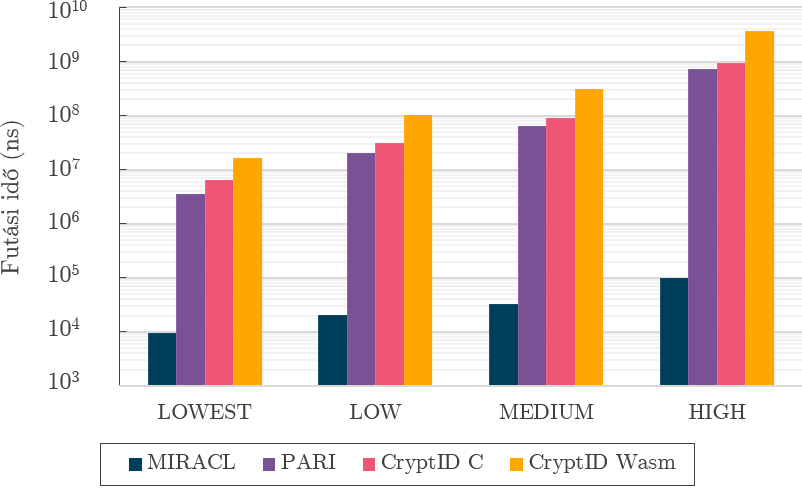
\includegraphics[height=225px]{05-cryptid/elliptic-multiplication-chart.png}
    \caption{Az elliptikus skaláris szorzás futási ideje.}
    \label{Figure::CryptID::EllipticMultiplicationChart}
\end{figure}

Az \dotref{Figure::CryptID::EllipticMultiplicationChart} ábrán logaritmikus skálára vetítve láthatjuk az egyes megoldások futási idejét különböző méretű bemenetekre. Az adatokból leolvasható, hogy az elvárásaink javarészt beigazolódtak: a MIRACL minden bemenet esetén nagyságrendekkel gyorsabban fut, mint a többi megoldás, és valóban a WebAssembly végrehajtása tart a legtovább. A MIRACL kitűnő teljesítményét többek között az implementált \textit{wNAF} algoritmus hatékonyságának köszönheti\footnote{\url{http://bit.ly/miracl-ecurve-mult}} \cite{ECCScalarMultiplicationAnalysis}, míg a WebAssembly lomhaságát feltehetőleg a szabvány fiatal volta okozta optimalizációs hiányosságok eredményezhetik. Utóbbi azt jelenti, hogy a WebAssembly verzió a legkisebb bemenet esetén két és félszer, a legnagyobb esetén pedig megközelítőleg négyszer annyi ideig fut, mint a natív bináris.

Kiemelendő ugyanakkor, hogy a PARI és a CryptID C teljesítményében nincs jelentős eltérés. Ennek hátterében az állhat, hogy a CryptID-hez hasonlóan a PARI is a GMP könyvtárra épül, valamint ugyanazt az algoritmust, az úgynevezett \textit{Double-and-Add} módszert implementálja\footnote{\url{http://bit.ly/pari-fpe-mul}} a skaláris szorzáshoz.

Érdemes azt is kihangsúlyozni, hogy ugyan a CryptID WebAssembly teljesítménye meg sem közelíti a MIRACL eredményét, azonban ennek esetében sem beszélhetünk elviselhetetlenül lassú futásról: \texttt{LOWEST} bemenetre ez $0{,}016$, míg \texttt{HIGH} bemenetre $3{,}732$ másodpercet jelent.

\paragraph{Optimalizációs lehetőségek}

A CryptID skaláris szorzás tekintetében nyújtott teljesítménye javítható a MIRACL által is használt \textit{wNAF} algoritmus megvalósításával. Ennek segítségével a könyvtár a futási időt tekintve feltehetően a MIRACL és a PARI között helyezkedne el. Habár a fejlesztést már megkezdtük, jelenleg még nem áll rendelkezésünkre tesztelhető kód.

További sebességnövekedés érhető el ezen felül a Heuberger és Mazzoli által leírt szorzási eljárás implementálásával \citeyear{HeubergerMazzoli::ECCScalarMultiplication}. A \textit{wNAF} elkészítését követően ezt is ki szeretnénk próbálni.

\subsection{Tate párosítás}

A skaláris szorzás mellett az IBE megvalósítások hangsúlyos eleme valamilyen párosítás. Ahhoz, hogy a titkosítás és a visszafejtés minél gyorsabban kerüljön végrehajtásra, elengedhetetlen ennek hatékony megvalósítása.

Sajnos a párosítást tekintve csak a CryptID C és WebAssembly változatát tudtuk összehasonlítani. Ennek oka, hogy a CryptID az RFC 5091-ben leírt, úgynevezett módosított Tate párosításra épül, mely a már említett könyvtárak egyikében sem található meg közvetlenül. 

Felhasználva az előző mérés során szerzett tapasztalatokat, azt vártuk, hogy a WebAssembly változat háromszor-négyszer lassabb lesz, mint a natív.

\begin{figure}[h]
    \centering
    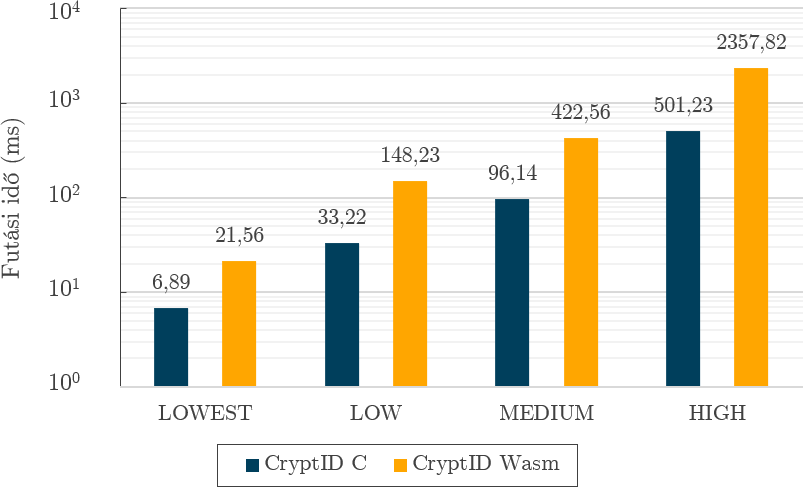
\includegraphics[height=225px]{05-cryptid/tate-pairing-chart.png}
    \caption{A Tate párosítás futási ideje.}
    \label{Figure::CryptID::TatePairingChart}
\end{figure}

Az \dotref{Figure::CryptID::TatePairingChart} ábra logaritmikus skálára vetítve mutatja a Tate párosítás különböző nagyságú bemeneteken mért futási idejét. Itt szeretnénk felhívni a figyelmet arra, hogy a grafikonon szereplő adatok ezúttal milliszekundumban kerültek rögzítésre. Az egyes sávok fölött található értékekből könnyen kiszámolható, hogy a WebAssembly bináris megközelítőleg háromszor-ötször tovább fut, mint a natív kód. A különbség tehát a skaláris szorzásnál mérthez hasonló.

Önmagában az ilyen mértékű sebességkülönbség jelenléte kellemetlennek tekinthető, azonban az eltérés konzisztens volta fontos bizonyíték arra vonatkozóan, hogy a WebAssembly környezet teljesítménye stabil, nem ingadozik.

\paragraph{Optimalizációs lehetőségek}

Az optimalizációra a Tate párosítás esetén két út kínálkozik: hatékonyabb algoritmus implementálása, illetve a meglevő algoritmus által hívott rutinok javítása. A következőkben az utóbbi lehetőséget tekintjük, azonban későbbi munkánk során szeretnénk algoritmikus módosításokat is megvizsgálni.

Az \dotref{Figure::CryptID::EncryptProfileChart} ábrán az \textit{Encrypt} teljesítményét meghatározó két függvény, a \texttt{TatePairing} \linebreak és a \texttt{HashToPoint} futási ideje szerepel egy \texttt{HIGH} bemenetre. A diagramon szereplő adatokból leolvasható, hogy a Tate párosítás teljesítménye mindenekelőtt a modulo hatványozást végző \texttt{modPow} és a multiplikatív inverzt számító \texttt{mulInv} futási idejének függvénye.

Úgy gondoljuk, hogy mindkét függvény teljesítményében jelentős előrelépés érhető el mikrooptimalizációk alkalmazásával. Ez a processzor \textit{cache} jobb kihasználását, a függvényhívások számának minimalizálását, valamint a függvényparaméterek és visszatérési értékek hatékonyabb kezelését foglalhatja például magában.

\subsection{Identity-based Encryption}

A két legfontosabb alaprutin áttekintése után következhet az Identity-based Encryptiont alkotó függvények (\textit{Setup, Encrypt, Extract, Decrypt}) teljesítményének elemzése. Tekintve, hogy a \textit{Setup} és az \textit{Extract} inkább szerveroldalon kerülhet felhasználásra, ezek esetében csupán a natív C és a Node.js-ben futtatott Wasm verziót hasonlítottuk össze. Az \textit{Encrypt} és a \textit{Decrypt} futási idejét azonban ezeken felül egy asztali és egy mobilos böngészőben is megmértük.

\subsubsection{Setup}

A \textit{Setup} függvény segítségével új publikus paramétereket és mesterkulcsot állíthatunk elő. Ezek generálása nem tekinthető olyan gyakori tevékenységnek, mint a titkosítás, a visszafejtés vagy a privát kulcs kinyerés. Ennélfogva a \textit{Setup} teljesítményével szemben támasztott elvárásaink kevésbé voltak szigorúak.

\begin{figure}[h]
    \centering
    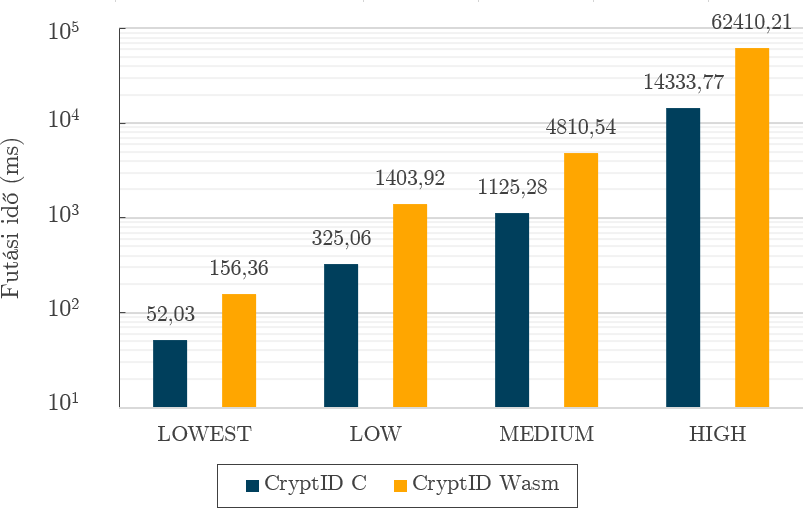
\includegraphics[height=225px]{05-cryptid/setup-chart.png}
    \caption{A \textit{Setup} függvény futási ideje.}
    \label{Figure::CryptID::SetupChart}
\end{figure}

A \textit{Setup} különböző nagyságú bemeneteken mért futási idejét az \dotref{Figure::CryptID::SetupChart} ábrán láthatjuk. Az egyes futási idők már egészen más nagyságrendben mozognak, mint például a skaláris szorzás esetén: a WebAssembly verzió \texttt{HIGH} bementre már több mint egy percig futott! Mi több, ugyanezen bemeneten a C változat is megközelítőleg $15$ másodpercig dolgozott.

\paragraph{Optimalizációs lehetőségek}

A \textit{Setup} teljesítményét a megfelelő értékek generálása határozza meg. Ennek folytán a futási idő javítható a generálási folyamat optimalizálásával, vagy a generált értékek számának csökkentésével. Utóbbi megoldás minimális befektetéssel kínál nagyságrenddekkel jobb teljesítményt, emiatt például a MIRACL is rögzít bizonyos elliptikus görbe paramétereket. Úgy gondoljuk, hogy ez a CryptID számára is megfelelő előrelépési lehetőség lenne, azonban még meg kell határoznunk azokat az értékeket, melyeket a kódban rögzíthetünk.

\subsubsection{Extract}

Az \textit{Extract} függvény a privát kulcsok kinyerésére szolgál. Ezt a feladatot a PKG végzi, aminek következtében \textit{Setuphoz} hasonlóan az \textit{Extract} esetén is elsősorban szerveroldali felhasználással számoltunk. Alapvető eltérés ugyanakkor, hogy az \textit{Extract} végrehajtási gyakorisága előreláthatólag jóval meghaladja a \textit{Setupnál} feltételezhetőt. Ennek folytán a futási ideje is kellőképpen alacsony kell, hogy legyen. 

\begin{figure}[h]
    \centering
    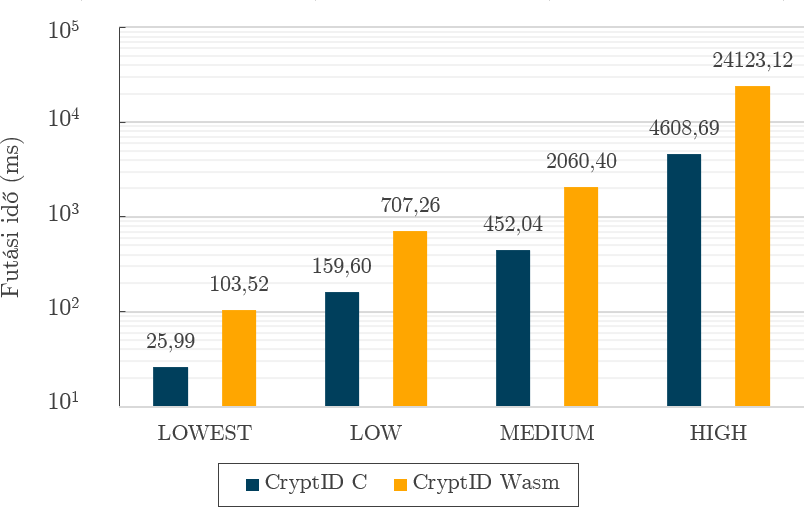
\includegraphics[height=225px]{05-cryptid/extract-chart.png}
    \caption{Az \textit{Extract} függvény futási ideje.}
    \label{Figure::CryptID::ExtractChart}
\end{figure}

Az \dotref{Figure::CryptID::ExtractChart} ábra a \textit{Extract} függvény futási idejét jeleníti meg. Míg a \texttt{LOWEST}, a \texttt{LOW} és a \texttt{MEDIUM} bemenetek esetén kielégítő értékekről beszélhetünk még a WebAssembly binárist tekintve is (legfeljebb $2$ másodperc), addig a \texttt{HIGH} bemenethez tartozó eredmények már meghaladják a kívánatosnak gondolt $1$–$2$ másodperces határt. A Wasm verzió különösen rossz, mintegy $24$ másodperces eredménnyel rendelkezik.

\paragraph{Optimalizációs lehetőségek}

Az \textit{Extract} futási idejét befolyásoló egyetlen komponens a \texttt{HashToPoint} eljárás. Az \dotref{Figure::CryptID::EncryptProfileChart} ábráról leolvasható, hogy ennek teljesítményét a skaláris szorzást megvalósító \texttt{affineMul} dominálja. Ez azt jelenti, hogy az \textit{Extract} futási idejét a skaláris szorzás felgyorsításával tudjuk javítani.

\subsubsection{Encrypt}

A titkosítást megvalósító \textit{Encrypt} függvény futását már egy asztali, valamint egy mobilos böngészőben is lemértük. Ennek oka, hogy a titkosítás kifejezetten egy kliensoldali műveletnek tekinthető, és ennek megfelelően legtöbbször a böngészőben kerül majd végrehajtásra. A hatékony implementáció ezúttal kiemelt fontosságot nyer, hiszen a mobil eszközök csak korlátozott erőforrásokkal rendelkeznek.

\begin{figure}[h]
    \centering
    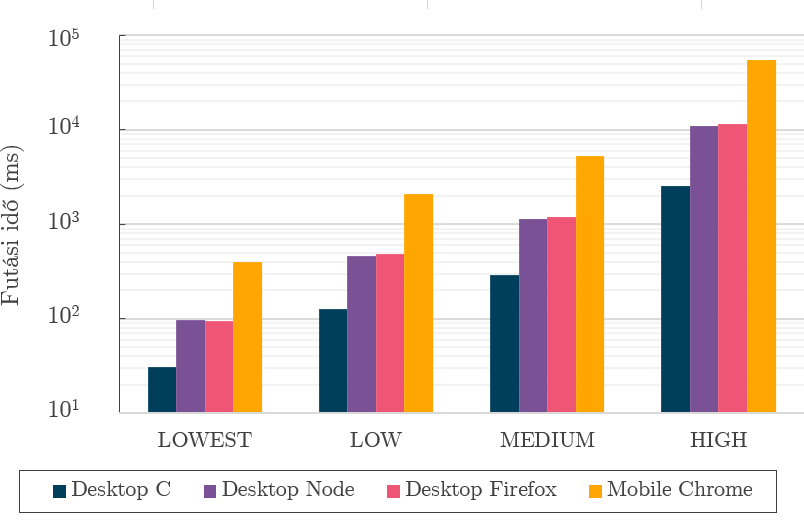
\includegraphics[height=225px]{05-cryptid/encrypt-chart.png}
    \caption{Az \textit{Encrypt} függvény futási ideje.}
    \label{Figure::CryptID::EncryptChart}
\end{figure}

A \dotref{Figure::CryptID::EncryptChart} ábrán ismét megfigyelhető a már látott tendencia: a Node.js-alapú WebAssembly háromszor-négyszer nagyobb értékeket produkál, mint a natív kód. Megjelenik emellett az asztali Firefox böngésző, mely nagy meglepetésünkre a Node.js-szel megegyező idők alatt futtatja a függvényt. Ez számunkra egy váratlan fordulat volt, hiszen előzetesen azt vártuk, hogy a böngésző, mint összetettebb beágyazó környezet, a Node.js-nél alacsonyabb teljesítményt fog biztosítani.

Sajnos a mobilos böngészőben történő végrehajtás jelentősen leszakad a többi értéktől: mintegy négyszer-ötször lassabb, mint az asztali WebAssembly. Ennek hátterében természetesen az architekturális, valamint erőforrásbeli különbségeket érdemes keresnünk.

\paragraph{Optimalizációs lehetőségek}

A könyvtárt integráló alkalmazások felhasználói élményét jelentősen befolyásolja a két legtöbbet használt függvény, az \textit{Encrypt} és a \textit{Decrypt} futási ideje. Ennek folytán kiemelt figyelemmel érdemes kezelni az ezekben adódó optimalizációs lehetőségeket.

A \dotref{Figure::CryptID::EncryptProfileChart} ábrán az \textit{Encrypt} egy futása során gyűjtött adatokat láthatunk. A bal oldali kördiagram az \textit{Encrypt} által hívott függvények végrehajtási idejét ábrázolja a teljes futási időhöz képest. Erről egyértelműen leolvasható, hogy a teljesítményt a \texttt{TatePairing} és a \texttt{HashToPoint} eljárás határozza meg. Ezen függvények összetevőit a jobb oldali kördiagramok ábrázolják.

Az \textit{Encrypt} sebessége tehát a Tate párosításnál ismertetett módszerek segítségével, valamint a \texttt{HashToPoint} függvényben szerepet játszó skaláris szorzás felgyorsításával növelhető.

\begin{figure}[h]
    \centering
    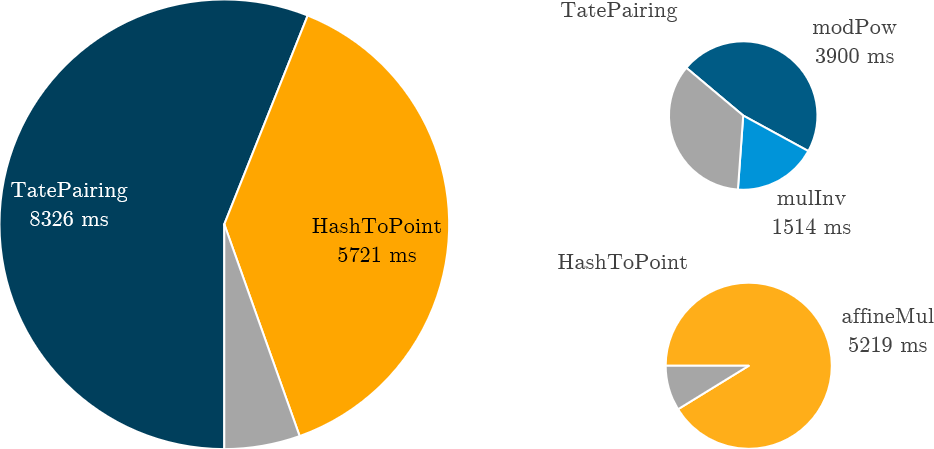
\includegraphics[height=210px]{05-cryptid/encrypt-profile-chart.png}
    \caption{Az \textit{Encrypt} függvényt alkotó komponensek futási ideje egy \texttt{HIGH} bemenetre (Desktop Firefox környezet).}
    \label{Figure::CryptID::EncryptProfileChart}
\end{figure}

\subsubsection{Decrypt}

Az \textit{Encrypthez} hasonlóan a \textit{Decrypt} futási idejét is négy környezetben mértük. Elvárásainkat az előző mérések vezérelték: úgy gondoltuk, hogy a natív C változat lesz a leggyorsabb, azonos időt ad a Desktop Node.js és a Firefox, a sort pedig a mobilos Chrome zárja. 

\begin{figure}[h]
    \centering
    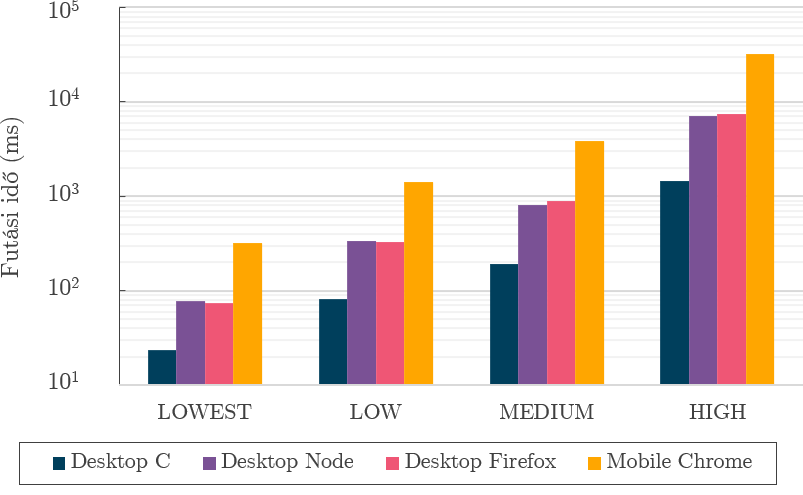
\includegraphics[height=225px]{05-cryptid/decrypt-chart.png}
    \caption{A \textit{Decrypt} függvény futási ideje.}
    \label{Figure::CryptID::DecryptChart}
\end{figure}

Az \dotref{Figure::CryptID::DecryptChart} ábráról leolvasható adatok pontosan az említett elvárásokat igazolják: az \textit{Encryptnél} látott relatív különbségek jelennek meg itt is. Felfedezhető a hasonlóság mindamellett az abszolút futási időt tekintve is: a \textit{Decrypt} végrehajtási ideje megközelítőleg $\frac{2}{3}$-a az \textit{Encryptének}. Ez a párhuzam abból adódik, hogy a \textit{Decrypt} sebességét szinte kizárólag a \texttt{TatePairing} határozza meg, \texttt{HashToPoint} hívás viszont ezúttal nincsen. 

\paragraph{Optimalizációs lehetőségek}

A \textit{Decrypt} teljesítményét a Tate párosítás dominálja, így ennek javítása tekinthető a legígéretesebb optimalizációs lehetőségnek.

\subsection{Összegzés}

A CryptID alapjául szolgáló legfontosabb rutinok teljesítményét látva kijelenthető, hogy asztali környezetben a könyvtár használhatónak tekinthető még nagyobb bemenet esetén is, mobil eszközökön azonban csak kisebb bemenetekre várhatunk kielégítő végrehajtási időt. Érdemes azonban ezen értékeléshez hozzátenni, hogy ezt a teljesítményt a CryptID javarészt egyszerűbb algoritmusok kevésbé hatékony megvalósításaival éri el. Emiatt számos, az előzőekben is felsorolt optimalizációs lehetőség adódik, melyek alkalmazásával a könyvtár teljesítménye jelentősen növelhető, megfelelő futási időt nyújtva mobil eszközökön is.
